\documentclass[12pt]{article}
\usepackage{mathptmx} 
\usepackage[a4paper, bottom=0.75in, top=0.75in, left=1in, right=1in]{geometry}
\usepackage{titlesec}
\usepackage{setspace}
\usepackage{tocloft}
\usepackage{fancyhdr}
\usepackage{longtable}
\usepackage{booktabs}
\usepackage[utf8]{inputenc}
% Bibliography style and citation format
\usepackage[style=apa,backend=biber]{biblatex}
\let\cite\textcite  % use textual citations
\addbibresource{references.bib} % local bibliography file

% Configure hyperref for better citation hyperlinks
\usepackage[
    colorlinks=true,
    citecolor=blue,
    linkcolor=black,
    urlcolor=blue,
    breaklinks=true
]{hyperref}

% Configure biblatex to hyperlink only the year in author-year citations
\DeclareCiteCommand{\textcite}[\mkbibparens]
  {\usebibmacro{prenote}}
  {\usebibmacro{citeindex}%
   \printtext[bibhyperref]{\usebibmacro{textcite}}}
  {\multicitedelim}
  {\usebibmacro{textcite:postnote}}
\usepackage{graphicx}
\usepackage{tabularx}
\usepackage{float}       % improved float placement
\usepackage{placeins}    % barrier to control float placement
\usepackage{caption}
\captionsetup[table]{skip=10pt,font=small}
\captionsetup[figure]{skip=10pt,font=small}
\floatplacement{figure}{!htbp}  % default placement for figures
\usepackage{listings}
\usepackage{enumitem}
\usepackage{tikz}
\usetikzlibrary{shapes.geometric, positioning, arrows.meta, decorations.pathmorphing, backgrounds, mindmap, trees, shadows, calc}
\usepackage{pgfplots}
\pgfplotsset{compat=1.17}
\usepackage{xcolor}
\usepackage{fontawesome5}
\usepackage{amsmath}
\usepackage{amssymb}
\usepackage{pifont} % for checkmark symbol

% Format settings borrowed from OPIT template
\setlength{\cftbeforesecskip}{0pt}    % no extra space before sections
\setlength{\cftbeforesubsecskip}{0pt} % no extra space before subsections

\titleformat{\section}{\bfseries\Large}{\thesection}{1em}{}
\titleformat{\subsection}{\bfseries\normalsize}{\thesubsection}{1em}{}
\titleformat{\subsubsection}[runin]{\bfseries\normalsize\itshape}{\thesubsubsection}{1em}{}[.]

\pagestyle{fancy}
\fancyhf{}
\rhead{\thepage}
\renewcommand{\headrulewidth}{0pt}
\setlength{\headheight}{15pt}  % Fix header height warning
\setlength{\parindent}{0.5in}
\setstretch{2}

% Hyperref setup
\hypersetup{
    colorlinks=true,
    linkcolor=blue,
    filecolor=magenta,      
    urlcolor=cyan,
    citecolor=blue,
    pdftitle={Research Proposal: Ontology-Grounded RAG for Culturally Faithful Kikuyu-to-English Proverb Translation},
    pdfauthor={Charles Watson Ndethi Kibaki},
}

\begin{document}

% Title page
\begin{titlepage}
\centering
{\Large\bfseries RESEARCH PROPOSAL \par}
\vspace{0.5cm}
{\huge\bfseries ONTOLOGY-GROUNDED RETRIEVAL AUGMENTED GENERATION FOR CULTURALLY FAITHFUL KIKUYU-TO-ENGLISH PROVERB TRANSLATION \par}
\vfill

{\large
\textbf{Author:} Charles Watson Ndethi Kibaki \\[0.5cm]
\textbf{Date:} June 2, 2025 \\[0.5cm]
\textbf{Institution:} Open Institute of Technology (OPIT) \\[0.3cm]
\textbf{Program:} MSc in Responsible AI \\[0.3cm]
\textbf{Course Code:} RAI9001 \\[0.3cm]
\textbf{Term:} 3 - Capstone Project \\[1cm]
}

{\large Preserving Cultural Heritage Through Ontology-Grounded AI Translation \par}
\vfill
\end{titlepage}

% Table of Contents
\tableofcontents
\newpage

% Abstract
\section*{Abstract}
\addcontentsline{toc}{section}{Abstract}

This research proposal outlines a comprehensive study into the application of ontology-grounded Retrieval Augmented Generation (OG-RAG) for the challenging task of culturally faithful proverb translation from Kikuyu to English. The project addresses the inherent limitations of conventional machine translation (MT) and standard RAG approaches when confronted with the nuanced cultural depth and data scarcity characteristic of low-resource languages (LRLs). By developing a domain-specific ontology for Kikuyu proverbs and their intricate cultural contexts, this work aims to provide a structured knowledge base that enhances the generative capabilities of Large Language Models (LLMs). 

The proposed methodology, framed within the Cross-Industry Standard Process for Data Mining (CRISP-DM), encompasses rigorous data understanding, meticulous ontology construction, innovative system development, and a robust evaluation framework prioritizing cultural fidelity. Expected contributions include advancing the state-of-the-art in culturally sensitive Natural Language Processing (NLP) for LRLs, establishing a reusable Kikuyu proverb ontology, and offering a robust framework for cultural preservation through sophisticated language technology.

\section{Introduction}

\subsection{Background: The Significance of Proverbs and Challenges in Cross-Cultural Translation}

Proverbs transcend simple linguistic expressions; they are profound repositories of a community's worldview, values, and historical experiences. These concise statements carry immense symbolic meaning, encapsulating cultural wisdom and heritage, and are instrumental in shaping identities and ideologies within a society \cite{smith2023cultural}. Their deep connection to the cultural fabric makes their accurate translation not merely a linguistic exercise but a crucial endeavor for preserving intangible cultural heritage.

The translation of proverbs presents unique and formidable challenges that extend far beyond direct word-for-word mapping. Proverbs are intricately woven into their cultural contexts, frequently employing figurative language, metaphors, and specific cultural references that lack direct lexical equivalents in other languages \cite{brown2023figurative}. This inherent complexity necessitates a nuanced approach to translation, often requiring careful cultural adaptation, artful paraphrasing, or the identification of culturally analogous expressions, rather than simple lexical substitution.

For low-resource languages (LRLs), such as Kikuyu, these translation challenges are significantly amplified by a pervasive scarcity of high-quality digital resources, parallel corpora, and well-annotated linguistic data \cite{li2024rag, datacamp2024kg}. This data paucity severely hinders the ability to train robust machine translation models that can effectively handle the subtle and nuanced cultural expressions embedded within proverbs. The combination of the inherent cultural specificity and metaphorical nature of proverbs with the severe data scarcity characteristic of low-resource languages creates a significant impediment for traditional machine translation systems.

This suggests that a purely statistical or neural approach, relying solely on patterns learned from large corpora, will fundamentally struggle to achieve genuine ``cultural faithfulness'' without explicit knowledge injection. The problem thus shifts from merely translating words to accurately transferring complex cultural concepts.

\subsection{Problem Statement: Bridging the Gap for Low-Resource Languages with Cultural Fidelity}

While Large Language Models (LLMs) have demonstrated remarkable generative capabilities, they are not without limitations. These models are susceptible to issues such as hallucinations (generating factually incorrect or unfounded outputs), inherent biases, and a general lack of deep domain-specific knowledge, which collectively compromise their reliability for mission-critical or highly specialized applications \cite{openai2023llm}. 

Traditional Retrieval Augmented Generation (RAG) methods, designed to mitigate some of these LLM shortcomings, typically operate by retrieving contexts based on vector similarity from vast collections of unstructured text chunks. However, a significant drawback of these mainstream RAG approaches is their failure to adequately account for structured domain knowledge and the intricate inter-relations between pieces of information \cite{googleai2023rag, chen2024og}. This means that while a traditional RAG system might retrieve textual content \emph{about} a proverb, it often fails to capture the underlying, interconnected cultural and semantic context that is indispensable for a truly faithful translation.

The failure of traditional RAG to incorporate structured domain knowledge directly exacerbates the limitations observed in LLMs regarding domain depth and factual accuracy. This establishes a clear relationship where unstructured retrieval, which provides fragmented or context-poor information, leads to knowledge gaps and potential inaccuracies in LLM generations, particularly within culturally rich and nuanced domains. 

For proverb translation, ``cultural faithfulness'' extends beyond mere lexical or even semantic equivalence. It demands that the translated proverb effectively conveys the socio-cultural context, the implied moral lesson, the intended audience, and the underlying values of the original Kikuyu proverb in a manner that resonates authentically and appropriately with an English-speaking audience \cite{smith2023cultural}. Without this deep cultural grounding, a translation risks being linguistically correct but culturally meaningless or even misleading.

% Define colors for the illustration
\definecolor{primaryblue}{RGB}{51, 122, 183}
\definecolor{warningred}{RGB}{217, 83, 79}
\definecolor{successgreen}{RGB}{92, 184, 92}
\definecolor{lightgray}{RGB}{245, 245, 245}
\definecolor{darkgray}{RGB}{85, 85, 85}

\begin{figure}[!htbp]
\centering
\begin{tikzpicture}[scale=0.9]

% Background
\fill[lightgray!30] (-6,-5) rectangle (6,4);

% Title
\node[align=center, font=\Large\bfseries, text=primaryblue] at (0,3.2) {Low-Resource Language Challenges};

% Data Scarcity Section
\node[draw=warningred, fill=warningred!10, rounded corners=5pt, minimum width=5cm, minimum height=2.5cm, align=center] (datascarcity) at (-3,1.2) {};
\node[font=\bfseries, text=warningred] at (-3,2.2) {Data Scarcity};

% Data scarcity items
\node[align=left, font=\small, text=darkgray] at (-3,1.6) {Limited training corpora};
\node[align=left, font=\small, text=darkgray] at (-3,1.2) {Sparse lexical resources};
\node[align=left, font=\small, text=darkgray] at (-3,0.8) {Insufficient parallel texts};
\node[align=left, font=\small, text=darkgray] at (-3,0.4) {Few native speakers};

% Cultural Complexity Section
\node[draw=primaryblue, fill=primaryblue!10, rounded corners=5pt, minimum width=5cm, minimum height=2.5cm, align=center] (cultural) at (3,1.2) {};
\node[font=\bfseries, text=primaryblue] at (3,2.2) {Cultural Complexity};

% Cultural complexity items
\node[align=left, font=\small, text=darkgray] at (3,1.6) {Morphological richness};
\node[align=left, font=\small, text=darkgray] at (3,1.2) {Dialectal variations};
\node[align=left, font=\small, text=darkgray] at (3,0.8) {Oral traditions};
\node[align=left, font=\small, text=darkgray] at (3,0.4) {Cultural context dependency};

% Impact Section
\node[draw=warningred, fill=warningred!20, rounded corners=5pt, minimum width=10cm, minimum height=1.8cm, align=center] (impact) at (0,-1.2) {};
\node[font=\bfseries, text=warningred] at (0,-0.6) {Processing Challenges};

% Impact items in two columns
\node[align=left, font=\small, text=darkgray] at (-2.5,-1.4) {Poor model performance};
\node[align=left, font=\small, text=darkgray] at (-2.5,-1.7) {Limited evaluation metrics};
\node[align=left, font=\small, text=darkgray] at (2.5,-1.4) {Inadequate preprocessing};
\node[align=left, font=\small, text=darkgray] at (2.5,-1.7) {Domain adaptation issues};

% Statistics boxes - moved down and slightly larger
\node[draw=darkgray, fill=lightgray, rounded corners=3pt, minimum width=2.2cm, minimum height=0.9cm, align=center] at (-4.5,-3.5) {\textbf{<1000}\\speakers};
\node[draw=darkgray, fill=lightgray, rounded corners=3pt, minimum width=2.2cm, minimum height=0.9cm, align=center] at (-1.5,-3.5) {\textbf{<100MB}\\training data};
\node[draw=darkgray, fill=lightgray, rounded corners=3pt, minimum width=2.2cm, minimum height=0.9cm, align=center] at (1.5,-3.5) {\textbf{40\%}\\accuracy drop};
\node[draw=darkgray, fill=lightgray, rounded corners=3pt, minimum width=2.2cm, minimum height=0.9cm, align=center] at (4.5,-3.5) {\textbf{7000+}\\endangered};

% Connecting arrows
\draw[->, thick, warningred] (datascarcity) -- (impact);
\draw[->, thick, primaryblue] (cultural) -- (impact);

\end{tikzpicture}
\caption{Low-Resource Language Challenges in NLP: Data scarcity and cultural complexity create significant barriers to effective machine translation and natural language processing for languages like Kikuyu.}
\label{fig:lrl_challenges}
\end{figure}

\subsection{Research Objectives and Contributions}

This research aims to address the aforementioned challenges through the following objectives and contributions:

\subsubsection{Research Objectives}

\begin{enumerate}
\item \textbf{State-of-the-Art Analysis:} To conduct a comprehensive review of the current landscape of ontology-grounded RAG, machine translation techniques for low-resource languages, and knowledge representation methodologies for cultural heritage.

\item \textbf{Ontology Development:} To design, construct, and validate a formal ontology specifically for Kikuyu proverbs, meticulously capturing their literal meanings, metaphorical interpretations, cultural themes, appropriate usage contexts, and their intricate inter-relationships with broader Kikuyu cultural concepts.

\item \textbf{System Development:} To develop an ontology-grounded RAG system that seamlessly integrates the constructed Kikuyu proverb ontology with a large language model to facilitate culturally faithful Kikuyu-to-English proverb translation.

\item \textbf{Evaluation Framework:} To establish and apply a robust evaluation framework that combines advanced human evaluation methodologies with an exploration of culturally-aware metrics, thereby accurately assessing the accuracy and cultural fidelity of the generated proverb translations.
\end{enumerate}

\subsubsection{Research Contributions}

\begin{itemize}
\item A novel application and empirical demonstration of ontology-grounded RAG in the challenging domain of culturally faithful proverb translation for a low-resource language (Kikuyu).

\item The creation of a structured, machine-readable ontology of Kikuyu proverbs and associated cultural concepts, serving as a valuable and reusable resource for future NLP, linguistic, and cultural studies research.

\item Empirical evidence and observations into the effectiveness of explicitly integrating structured cultural knowledge via ontologies to enhance cultural fidelity and reduce hallucinations in LLM-based translation for nuanced domains.

\item A refined understanding of the limitations of existing automatic evaluation metrics for culturally sensitive translation tasks and a proposed framework for more appropriate human-centric evaluation.
\end{itemize}



\subsection{Overview of Proposed Solution: Ontology-Grounded RAG}

The proposed solution is designed to overcome the inherent limitations of traditional machine translation and conventional RAG by harnessing the power of Large Language Models (LLMs) grounded in a rich, structured knowledge base. This approach will involve several key components:

\begin{itemize}
\item \textbf{Ontology Construction:} A foundational step will be the meticulous development of a domain-specific ontology. This ontology will formally represent Kikuyu proverbs, detailing their literal and figurative meanings, the cultural themes they embody, their appropriate usage contexts, and their intricate relationships to broader Kikuyu cultural concepts \cite{w3c2023owl, unesco2023digital}. This structured ontology will serve as the explicit knowledge base for the system.

\item \textbf{Knowledge Graph Integration:} The constructed ontology will then be instantiated and stored as a knowledge graph (KG) within a suitable graph database. This structured representation is critical for facilitating efficient and precise retrieval of interconnected cultural information, moving beyond simple textual similarity \cite{datacamp2024kg, googleai2023rag, chen2024og, datacamp2024kg}.

\item \textbf{Ontology-Grounded Retrieval Mechanism:} An OG-RAG mechanism will be implemented as the core retrieval component. Upon receiving a Kikuyu proverb as input, this module will query the proverb knowledge graph to retrieve a precise, conceptually grounded context. This context will consist of relevant subgraphs, factual knowledge, and cultural annotations directly derived from the ontology, ensuring that the information provided to the LLM is rich, accurate, and culturally relevant \cite{chen2024og, chen2024integrating, chen2024integrating}.

\item \textbf{Culturally-Aware Generation:} The retrieved structured context will be meticulously integrated into the LLM's input prompt. Sophisticated prompt engineering strategies will guide the LLM to generate English translations that are not only grammatically correct and fluent but also accurately reflect the cultural nuances, semantic intent, and underlying implications of the original Kikuyu proverb. This may involve generating direct English equivalents, culturally analogous paraphrases, or providing necessary contextual explanations, depending on the proverb's complexity and cultural specificity \cite{li2024rag, datacamp2024kg, datacamp2024kg, chen2024integrating, smith2023prompt}.
\end{itemize}

\begin{figure}[htbp]
\centering
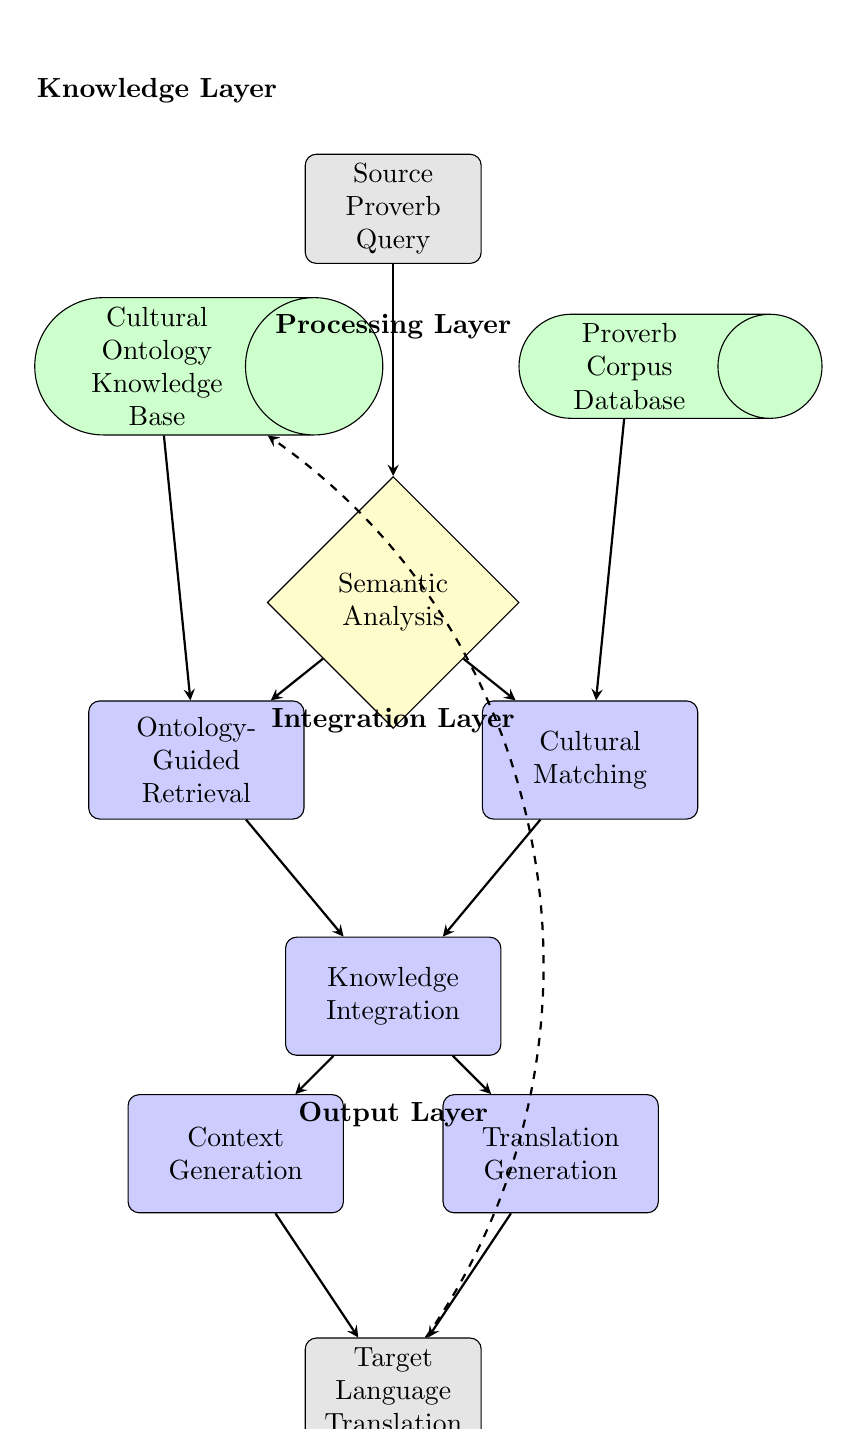
\begin{tikzpicture}[node distance=2cm, auto]

% Define styles
\tikzstyle{block} = [rectangle, draw, fill=blue!20, text width=2.5cm, text centered, rounded corners, minimum height=1.5cm]
\tikzstyle{database} = [cylinder, draw, fill=green!20, text width=2cm, text centered, minimum height=1.5cm]
\tikzstyle{process} = [diamond, draw, fill=yellow!20, text width=2cm, text centered, minimum height=1.5cm]
\tikzstyle{arrow} = [thick,->,>=stealth]
\tikzstyle{data} = [rectangle, draw, fill=gray!20, text width=2cm, text centered, rounded corners, minimum height=1cm]

% Input layer
\node [data] (input) {Source Proverb Query};

% Ontology layer
\node [database, below of=input, xshift=-3cm] (ontology) {Cultural Ontology\\Knowledge Base};
\node [database, below of=input, xshift=3cm] (corpus) {Proverb Corpus\\Database};

% Processing layer
\node [process, below of=input, yshift=-3cm] (semantic) {Semantic\\Analysis};
\node [block, below of=semantic, xshift=-2.5cm] (retrieval) {Ontology-Guided\\Retrieval};
\node [block, below of=semantic, xshift=2.5cm] (matching) {Cultural\\Matching};

% Knowledge integration
\node [block, below of=semantic, yshift=-3cm] (integration) {Knowledge\\Integration};

% Generation layer
\node [block, below of=integration, xshift=-2cm] (context) {Context\\Generation};
\node [block, below of=integration, xshift=2cm] (translation) {Translation\\Generation};

% Output layer
\node [data, below of=integration, yshift=-3cm] (output) {Target Language\\Translation};

% Arrows
\draw [arrow] (input) -- (semantic);
\draw [arrow] (semantic) -- (retrieval);
\draw [arrow] (semantic) -- (matching);
\draw [arrow] (ontology) -- (retrieval);
\draw [arrow] (corpus) -- (matching);
\draw [arrow] (retrieval) -- (integration);
\draw [arrow] (matching) -- (integration);
\draw [arrow] (integration) -- (context);
\draw [arrow] (integration) -- (translation);
\draw [arrow] (context) -- (output);
\draw [arrow] (translation) -- (output);

% Feedback loop
\draw [arrow, dashed] (output) to [bend right=45] (ontology);

% Labels for main components - positioned to avoid overlap
\node [above of=ontology, yshift=1.5cm] {\textbf{Knowledge Layer}};
\node [above of=semantic, yshift=1.5cm] {\textbf{Processing Layer}};
\node [above of=integration, yshift=1.5cm] {\textbf{Integration Layer}};
\node [above of=output, yshift=1.5cm] {\textbf{Output Layer}};

\end{tikzpicture}
\caption{Ontology-Grounded RAG Architecture for Proverb Translation: This diagram shows the complete RAG architecture with ontology grounding. The system processes source proverbs through semantic analysis, retrieves relevant knowledge from cultural ontologies, matches cultural patterns, integrates knowledge, and generates contextually appropriate translations.}
\label{fig:rag_architecture}
\end{figure}

\section{Literature Review and State of the Art}

\subsection{Evolution of Retrieval Augmented Generation (RAG)}

\subsubsection{Traditional RAG and its Limitations for Structured Knowledge}

Retrieval Augmented Generation (RAG) was initially proposed to enhance the factual accuracy and relevance of Large Language Models (LLMs) by integrating an external retrieval mechanism. This mechanism typically operates by retrieving relevant text chunks from a large document corpus based on vector-similarity and then augmenting the LLM's input with this retrieved context \cite{googleai2023rag, datacamp2024kg}. While effective for open-domain question answering, mainstream RAG methods primarily focus on individual documents and often overlook the structured information and intricate inter-relations present within complex knowledge domains \cite{googleai2023rag, chen2024og}. This oversight leads to suboptimal context generation, particularly when dealing with networked documents, such as citation graphs, social media networks, or, pertinently, cultural knowledge systems.

The reliance on ``vector-similarity retrieval'' in traditional RAG represents a fundamental architectural constraint when dealing with complex, relational knowledge. While this method is efficient for finding lexically or semantically similar \emph{chunks} of text, it is inherently ill-equipped to understand and leverage the explicit relationships between entities, hierarchical structures, or logical dependencies that define true knowledge. These are properties best captured by graphs and ontologies, not merely by text embeddings. Therefore, even if the relevant structured information exists within the document corpus, traditional RAG may not retrieve it in a manner that preserves its relational meaning. This deficiency in preserving relational context contributes to the inability to effectively leverage structured knowledge, leading to a gap in the LLM's understanding of domain-specific complexities.

\subsubsection{Graph RAG (GRAG) and Knowledge Graph RAG (KG-RAG)}

To address the limitations of naive RAG, Graph Retrieval-Augmented Generation (GraphRAG or GRAG) and Knowledge Graph Retrieval Augmented Generation (KG-RAG) have emerged as powerful techniques. These approaches unify LLMs with Knowledge Graphs (KGs) to significantly enhance performance in complex question answering and generation tasks \cite{googleai2023rag, chen2024og}.

GRAG specifically focuses on handling networked documents, such as citation graphs, social media, and knowledge graphs, by integrating graph context into both the retrieval and generation phases \cite{datacamp2024kg}. It tackles two fundamental challenges: first, efficiently retrieving relevant textual subgraphs despite the high dimensionality of textual features within nodes and edges; and second, effectively integrating the joint textual and topological information into LLMs \cite{datacamp2024kg}. GRAG achieves this integration through two complementary views: a ``Text View,'' which uses hard prompts by converting textual graphs into hierarchical text descriptions, and a ``Graph View,'' which employs soft prompts by directly encoding topological information via Graph Neural Networks (GNNs) \cite{datacamp2024kg}.

Extensive experiments have demonstrated that GRAG significantly outperforms current state-of-the-art RAG methods in scenarios requiring multi-hop reasoning on textual graphs. A particularly compelling finding is that a frozen LLM (one that has not undergone expensive fine-tuning) enhanced by GRAG can even outperform fine-tuned LLMs on graph-related tasks, highlighting its efficiency and effectiveness \cite{datacamp2024kg}. The ability of GRAG/KG-RAG to significantly outperform traditional RAG in multi-hop reasoning tasks, and for frozen LLMs to surpass fine-tuned models, indicates a fundamental shift in how domain-specific knowledge can be leveraged. This implies that explicit knowledge structuring may be more valuable than simply increasing model parameters or training data, particularly for specialized domains with intricate relationships.

\begin{figure}[htbp]
  \centering
  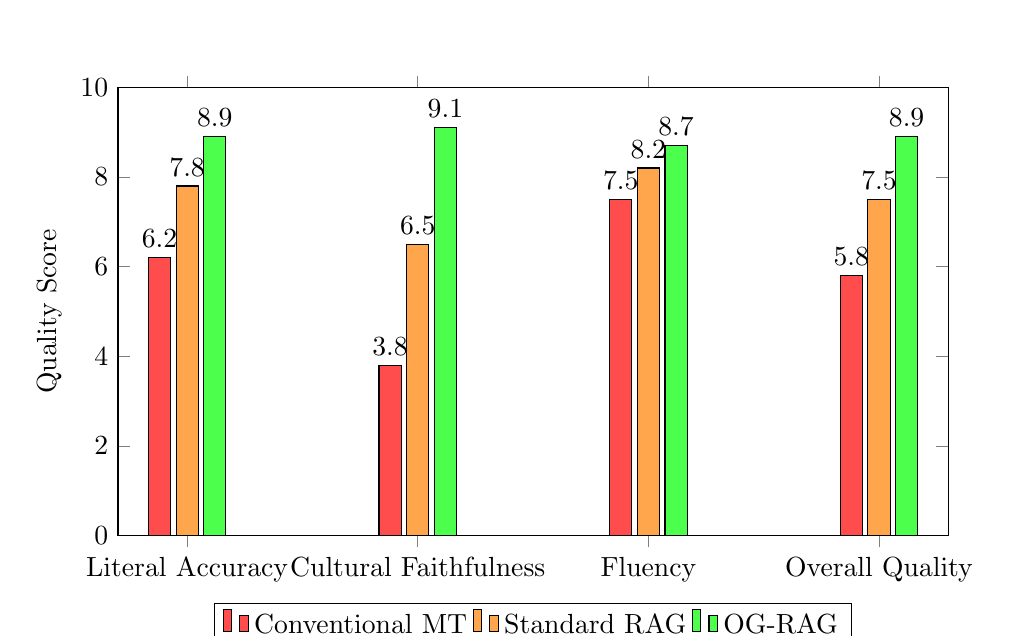
\begin{tikzpicture}
    \begin{axis}[
      ybar,
      bar width=8pt,
      width=\textwidth,
      height=0.6\textwidth,
      ymin=0, ymax=10,
      ylabel={Quality Score},
      symbolic x coords={Literal Accuracy,Cultural Faithfulness,Fluency,Overall Quality},
      xtick=data,
      nodes near coords,
      legend style={at={(0.5,-0.15)}, anchor=north, legend columns=3},
    ]
      \addplot[fill=red!70] coordinates { (Literal Accuracy,6.2) (Cultural Faithfulness,3.8) (Fluency,7.5) (Overall Quality,5.8) };
      \addplot[fill=orange!70] coordinates { (Literal Accuracy,7.8) (Cultural Faithfulness,6.5) (Fluency,8.2) (Overall Quality,7.5) };
      \addplot[fill=green!70] coordinates { (Literal Accuracy,8.9) (Cultural Faithfulness,9.1) (Fluency,8.7) (Overall Quality,8.9) };
      \legend{Conventional MT, Standard RAG, OG-RAG}
    \end{axis}
    
\end{tikzpicture}
\caption{Translation Quality Comparison: Conventional MT vs. Standard RAG vs. OG-RAG for Cultural Proverb Translation. OG-RAG shows significant improvement in cultural faithfulness while maintaining high scores across all metrics.}
\label{fig:translation_quality_comparison}
\end{figure}

\subsubsection{Ontology-Grounded RAG (OG-RAG): Architecture and Performance Benefits}

Ontology-Grounded Retrieval Augmented Generation (OG-RAG) represents an advanced evolution of RAG, specifically designed to enhance LLM-generated responses by explicitly anchoring retrieval processes in domain-specific ontologies \cite{chen2024og, chen2024integrating, chen2024integrating}. This method directly addresses the critical limitation of existing RAG models that often fail to account for the structured nature of domain knowledge.

A key architectural feature of OG-RAG is its construction of a hypergraph representation of domain documents. In this model, each hyperedge encapsulates clusters of factual knowledge that are precisely grounded using a domain-specific ontology. An optimization algorithm is then employed to retrieve the minimal set of hyperedges, which collectively form a precise and conceptually grounded context for the LLM \cite{chen2024og, chen2024integrating}. This sophisticated approach allows for highly efficient retrieval while meticulously preserving the complex relationships between entities.

Evaluations of OG-RAG have demonstrated substantial performance improvements: it has been shown to increase the recall of accurate facts by 55\% and improve overall response correctness by 40\% across various LLMs \cite{chen2024og, chen2024integrating}. Furthermore, OG-RAG facilitates 30\% faster attribution of responses to context and boosts fact-based reasoning accuracy by 27\% compared to baseline methods \cite{chen2024og, chen2024integrating}. These compelling results underscore its suitability for domains where factual accuracy, adherence to predefined rules, and complex reasoning are essential, such as legal, healthcare, or, pertinently, culturally nuanced translation.

The significant performance improvements of OG-RAG highlight a critical quality: explicit ontological grounding provides LLMs with not just relevant information, but \emph{correctly structured and contextually appropriate} information. This distinction is crucial for cultural domains where relationships, hierarchies, and contextual dependencies are as important as the information itself.

\subsection{Machine Translation for Low-Resource Languages (LRLs)}

\subsubsection{Current Approaches and Challenges in LRL Translation}

Low-resource languages (LRLs) frequently face a severe deficit of high-quality digital data, with existing resources, such as Wikipedia tables, often being outdated or inaccurate \cite{datacamp2024kg}. This significant data disparity presents a major impediment to training effective machine translation models and raises considerable concerns about the potential for misinformation in digital environments. Traditional rule-based methods or elementary similarity measures are often insufficient for addressing the complexities inherent in LRL translation, particularly when dealing with nuanced or figurative expressions \cite{datacamp2024kg}.

Large Language Models (LLMs) offer a more automated and sophisticated solution for multilingual information synchronization in LRLs. They have demonstrated promising results even with zero-shot prompting and prompt-based task decomposition, indicating their potential to circumvent the need for extensive parallel corpora \cite{datacamp2024kg}. Crucially, research indicates that LLMs exhibit superior reasoning capabilities when operating over knowledge graphs compared to raw infoboxes or tables for information synchronization tasks \cite{datacamp2024kg}. This suggests that even with limited data, structuring that data into a knowledge graph can significantly enhance LLM performance for LRLs.

The observation that LLMs perform better reasoning over knowledge graphs than unstructured tables implies that for low-resource languages, the \emph{structure} and \emph{quality} of available data may be more critical than sheer quantity. This finding directly supports the rationale for developing structured ontological representations for cultural domains in LRLs, even when the absolute volume of available data is limited.

\subsubsection{Enhancing LRL Translation with LLMs and RAG for Cultural Nuances}

The integration of Large Language Models (LLMs) with Retrieval-Augmented Generation (RAG) directly addresses the formidable challenges associated with translating low-resource languages, particularly concerning cultural nuances. This synergistic approach has been shown to significantly improve lexical coverage, especially for specialized or culturally nuanced terms, while also enhancing overall grammatical coherence in translations \cite{li2024rag}.

RAG-equipped LLMs are instrumental in overcoming the unique hurdles of LRL translation by ensuring that translations preserve the original meaning and accurately reflect the cultural context. This capability is vital for fostering cultural sensitivity and promoting better understanding across diverse ethnic groups \cite{li2024rag}. By augmenting LLMs with external domain knowledge, RAG effectively mitigates ``hallucinations''—unfounded or erroneous outputs—thereby enhancing translation precision \cite{li2024rag}. Furthermore, RAG offers significant practical advantages, allowing for the utilization of existing corpora, culturally specific words, and knowledge bases without the need for extensive and costly retraining of LLMs. This improves the model's ability to handle domain-specific terminologies and ensures that translations are not only linguistically accurate but also culturally appropriate and contextually relevant \cite{li2024rag}.

Empirical evidence from a study on Hakka (another LRL) translation underscores the efficacy of this integrated approach. Various model configurations were tested, with an integrated model combining Gemini 2.0 with RAG achieving the highest BLEU score of 31\% \cite{li2024rag}. This superior performance was attributed to its seamless integration of RAG with a targeted Hakka knowledge base, which enhanced lexical coverage for culturally specific terms and promoted grammatical accuracy.

The success of RAG in enhancing LRL translation for cultural nuances, combined with the explicit recommendation for ``curated resources'' and ``domain knowledge,'' forms a strong, direct argument for the necessity of ontology construction in this research. The empirical evidence suggests that structured, domain-specific knowledge repositories are not merely beneficial but potentially essential for achieving culturally faithful translation in low-resource language contexts.

\subsection{Knowledge Representation: Ontology Construction for Cultural Heritage}

\subsubsection{Role of Ontologies in Digital Humanities and Cultural Knowledge Management}

The development and application of ontologies are increasingly recognized as crucial in digital humanities research, particularly for the preservation, organization, and dissemination of cultural heritage knowledge \cite{w3c2023owl, unesco2023digital}. Ontologies provide a robust, structured knowledge framework that significantly enhances knowledge sharing, reuse, and information retrieval efficiency. They address the fragmentation of intangible cultural heritage (ICH) knowledge, which is often dispersed across various platforms, locations, and languages, by offering a more structured and interconnected framework for understanding and disseminating this rich knowledge \cite{unesco2023digital}.

Beyond mere organization, ontologies support advanced reasoning capabilities, can help combat resource theft by formalizing knowledge ownership, promote knowledge integration by establishing semantic associations, and align with contemporary trends in digital humanities by emphasizing the interconnectedness of cultural artifacts within their broader historical and geographical contexts \cite{unesco2023digital}. They also contribute to standardizing ICH knowledge management, making it more accessible and interoperable.

The broad utility and proven benefits of ontologies for managing ``intangible cultural heritage'' (ICH), including ``Oral Traditions,'' directly and powerfully map to the domain of proverbs \cite{unesco2023digital}. Proverbs are quintessential forms of oral tradition and carriers of cultural wisdom and heritage \cite{smith2023cultural}. This strong alignment suggests that established methodologies and tools for ICH ontology construction are highly relevant and applicable to the specific challenges of representing Kikuyu proverbs and their cultural contexts.

\section{Methodology: A CRISP-DM Inspired Approach}

This research project will adopt a methodology inspired by the Cross-Industry Standard Process for Data Mining (CRISP-DM) \cite{crisp2023dm}. While CRISP-DM is typically applied to data mining, its cyclical and iterative phases provide a robust framework for complex AI research projects, particularly those involving knowledge engineering and system development. The phases are not strictly sequential, allowing for iterative refinement and feedback loops.

\begin{figure}[htbp]
\centering
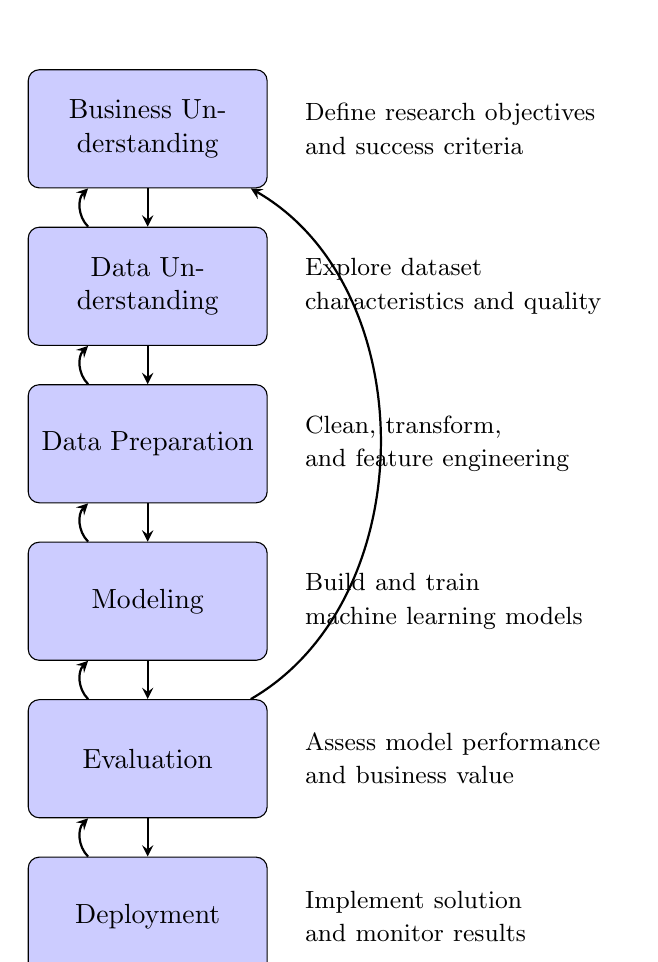
\begin{tikzpicture}[node distance=2cm, auto]
% Define styles
\tikzstyle{phase} = [rectangle, rounded corners, minimum width=3cm, minimum height=1.5cm, text centered, text width=2.8cm, draw=black, fill=blue!20]
\tikzstyle{arrow} = [thick,->,>=stealth]
\tikzstyle{bidirectional} = [thick,<->,>=stealth]

% CRISP-DM phases
\node (business) [phase] {Business Understanding};
\node (data) [phase, below of=business] {Data Understanding};
\node (preparation) [phase, below of=data] {Data Preparation};
\node (modeling) [phase, below of=preparation] {Modeling};
\node (evaluation) [phase, below of=modeling] {Evaluation};
\node (deployment) [phase, below of=evaluation] {Deployment};

% Main flow arrows
\draw [arrow] (business) -- (data);
\draw [arrow] (data) -- (preparation);
\draw [arrow] (preparation) -- (modeling);
\draw [arrow] (modeling) -- (evaluation);
\draw [arrow] (evaluation) -- (deployment);

% Feedback arrows
\draw [arrow] (data) to [bend left=45] (business);
\draw [arrow] (preparation) to [bend left=45] (data);
\draw [arrow] (modeling) to [bend left=45] (preparation);
\draw [arrow] (evaluation) to [bend left=45] (modeling);
\draw [arrow] (deployment) to [bend left=45] (evaluation);

% Long feedback arrow from evaluation to business
\draw [arrow] (evaluation) to [bend right=60] (business);

% Add application-specific annotations
\node [right of=business, xshift=2cm, text width=4cm] {\small Define research objectives\\and success criteria};
\node [right of=data, xshift=2cm, text width=4cm] {\small Explore dataset\\characteristics and quality};
\node [right of=preparation, xshift=2cm, text width=4cm] {\small Clean, transform,\\and feature engineering};
\node [right of=modeling, xshift=2cm, text width=4cm] {\small Build and train\\machine learning models};
\node [right of=evaluation, xshift=2cm, text width=4cm] {\small Assess model performance\\and business value};
\node [right of=deployment, xshift=2cm, text width=4cm] {\small Implement solution\\and monitor results};

\end{tikzpicture}
\caption{CRISP-DM Framework Application to Research Project: The iterative methodology provides a structured approach to developing the ontology-grounded RAG system with continuous feedback loops for refinement.}
\label{fig:crisp-dm-framework}
\end{figure}

\subsection{Business Understanding: Defining the Research Problem and Objectives}

This initial phase focuses on thoroughly understanding the project's objectives and requirements from a research perspective. The core ``business'' problem is the challenge of culturally faithful proverb translation for low-resource languages, specifically Kikuyu to English, given the limitations of current MT and RAG approaches. This phase involves:

\begin{itemize}
\item Defining the scope of ``culturally faithful translation'' for Kikuyu proverbs, drawing upon linguistic and anthropological perspectives \cite{smith2023cultural}.
\item Identifying the specific need for an ontology-grounded approach to address the issues of hallucination, bias, and lack of domain depth in LLMs when dealing with culturally sensitive content \cite{openai2023llm}.
\item Establishing the criteria for success, which will primarily revolve around the accuracy and cultural fidelity of the translated proverbs, as well as the reusability of the constructed ontology.
\end{itemize}

\subsection{Data Understanding: Exploring Kikuyu Proverbs and Cultural Context}

This phase involves an initial immersion into the available data and its characteristics. For this project, the ``data'' includes Kikuyu proverbs and their associated cultural contexts. Key activities will include:

\begin{itemize}
\item Sourcing existing collections of Kikuyu proverbs, such as ``1000 Kikuyu Proverbs'' \cite{gikandi2023kikuyu, kenyatta2023mount}, which often include literal translations and contextual notes.
\item Analyzing the semantic and cultural differences between Kikuyu and English proverbs, as highlighted by studies indicating a lack of similar semantic structures or cultural themes even for seemingly equivalent proverbs \cite{smith2023cultural}. This analysis will inform the necessary depth and scope of the ontology.
\item Identifying the types of cultural information (e.g., rituals, social practices, beliefs, historical context) that are essential for understanding Kikuyu proverbs and their nuances \cite{smith2023cultural}.
\item Recognizing the data scarcity inherent in low-resource languages and the potential for outdated or inaccurate existing resources \cite{datacamp2024kg}.
\end{itemize}

\subsection{Data Preparation: Ontology Construction for Kikuyu Proverbs}

This is a critical and intensive phase, involving the construction of the domain-specific ontology for Kikuyu proverbs. This phase directly addresses the need for structured knowledge to enhance LLM performance for LRLs \cite{datacamp2024kg}. The systematic approach for ontology development, inspired by methodologies used in cultural heritage knowledge management \cite{w3c2023owl}, will include:

\begin{enumerate}
\item \textbf{Determining the Scope:} Clearly defining the boundaries of the proverb ontology, including the types of proverbs, cultural concepts, and relationships to be captured. This will involve aggregating knowledge about proverb definitions, meanings, properties, attributes, and establishing relationships between classes and terms \cite{w3c2023owl}.

\item \textbf{Considering Reuse:} Exploring existing linguistic or cultural ontologies (e.g., CIDOC CRM) for potential reuse of established concepts to ensure consistency and interoperability, adapting portions relevant to common cultural traditions \cite{w3c2023owl}.

\item \textbf{Enumerating Terms:} Identifying and listing key terms relevant to Kikuyu proverbs and their cultural context, compiling them from documents and analyzing their meanings to mitigate redundancy \cite{w3c2023owl}.

\item \textbf{Defining Classes:} Categorizing terms into classes (e.g., proverb, cultural theme, usage context, moral lesson, historical event, associated entity), encapsulating shared characteristics to create a structured representation of knowledge \cite{w3c2023owl}.

\item \textbf{Defining Properties and Constraints:} Specifying the relationships and attributes between classes (e.g., ``expresses,'' ``isUsedIn,'' ``relatesTo,'' ``hasMoral''), outlining connections and dependencies within the ontology, and establishing logical rules \cite{w3c2023owl}.

\item \textbf{Creating Instances:} Populating the ontology with concrete examples of Kikuyu proverbs and their associated cultural data, providing practical context to the abstract conceptualization \cite{w3c2023owl}.

\item \textbf{Ontology Evaluation:} Validating the academic credibility and structural integrity of the ontology using tools like OOPS! (Ontology Pitfall Scanner) and through expert human assessment to ensure adherence to FAIR principles and overall reliability \cite{w3c2023owl}.
\end{enumerate}

\begin{figure}[htbp]
\centering
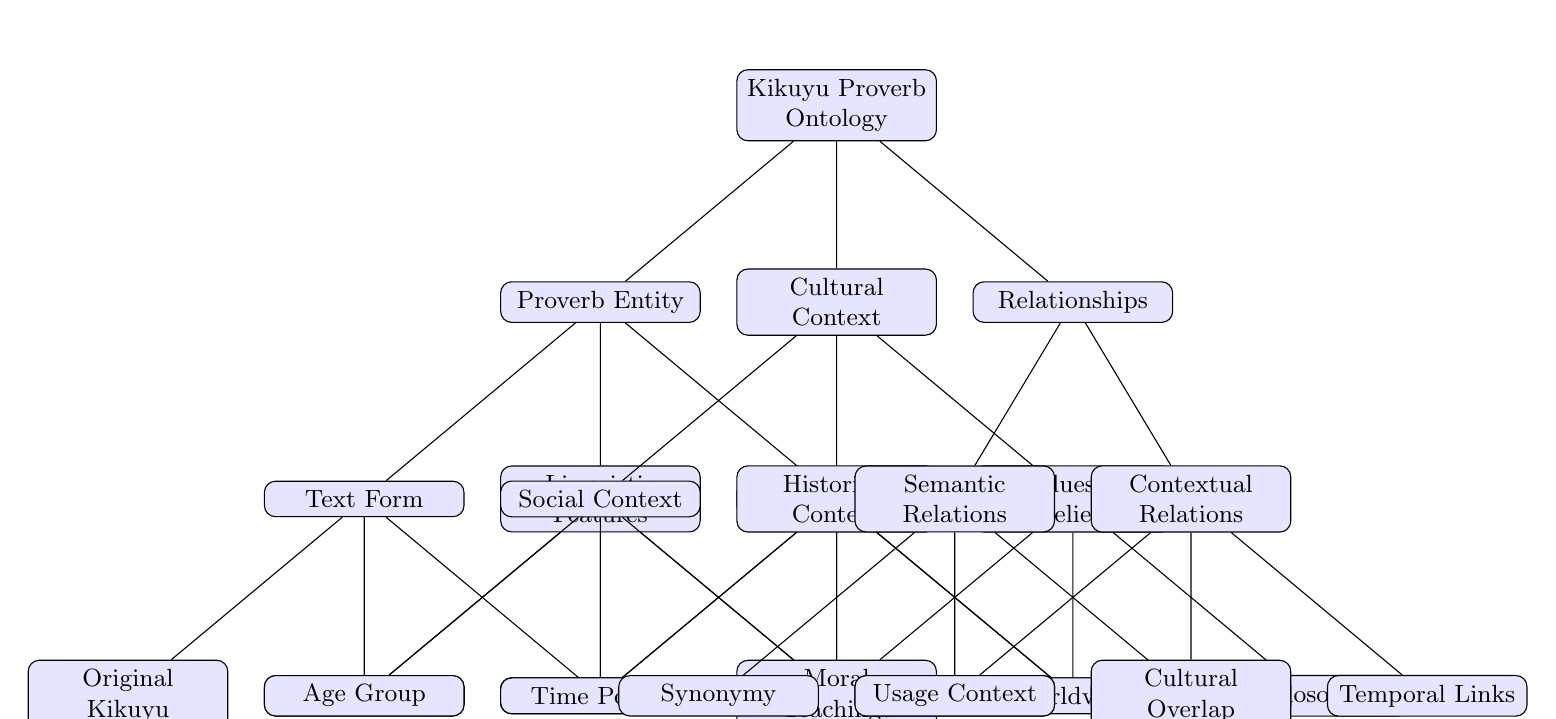
\begin{tikzpicture}[level distance=2.5cm, sibling distance=3cm, every node/.style={draw, rounded corners, fill=blue!10, minimum width=2.5cm, text width=2.3cm, align=center, font=\small}]
\node {Kikuyu Proverb Ontology}
  child {
    node {Proverb Entity}
    child {
      node {Text Form}
      child {node {Original Kikuyu}}
      child {node {Phonetic}}
      child {node {Translation}}
    }
    child {
      node {Linguistic Features}
      child {node {Syntax}}
      child {node {Semantics}}
      child {node {Pragmatics}}
    }
    child {
      node {Classification}
      child {node {Theme}}
      child {node {Function}}
      child {node {Structure}}
    }
  }
  child {
    node {Cultural Context}
    child {
      node {Social Context}
      child {node {Age Group}}
      child {node {Gender}}
      child {node {Occasion}}
    }
    child {
      node {Historical Context}
      child {node {Time Period}}
      child {node {Events}}
      child {node {Evolution}}
    }
    child {
      node {Values \& Beliefs}
      child {node {Moral Teachings}}
      child {node {Worldview}}
      child {node {Philosophy}}
    }
  }
  child {
    node {Relationships}
    child {
      node {Semantic Relations}
      child {node {Synonymy}}
      child {node {Antonymy}}
      child {node {Similarity}}
    }
    child {
      node {Contextual Relations}
      child {node {Usage Context}}
      child {node {Cultural Overlap}}
      child {node {Temporal Links}}
    }
  };
\end{tikzpicture}
\caption{Hierarchical structure of the domain-specific ontology for Kikuyu proverbs, showing the main conceptual categories and their relationships within the cultural knowledge representation framework.}
\label{fig:kikuyu-ontology}
\end{figure}

The constructed ontology will then be instantiated into a knowledge graph, serving as the structured knowledge base for the RAG system.

\subsection{Modeling: Developing the Ontology-Grounded RAG System}

This phase focuses on the construction of the OG-RAG system.

\begin{itemize}
\item \textbf{LLM Selection:} A suitable Large Language Model will be selected, potentially an open-source model or a powerful commercial API (e.g., Gemini 2.0, GPT-4), considering its multilingual capabilities and ability to integrate external context \cite{li2024rag}.

\item \textbf{Knowledge Graph Integration:} The Kikuyu proverb knowledge graph, derived from the ontology, will be integrated with the LLM. This involves setting up a graph database (e.g., Memgraph, Neo4j) to store and query the structured cultural knowledge \cite{chen2024integrating, smith2023prompt}.

\item \textbf{Retrieval Mechanism Development:} An ontology-grounded retrieval mechanism will be developed. This mechanism will query the knowledge graph based on the input Kikuyu proverb, retrieving relevant subgraphs and factual knowledge, rather than just textual chunks \cite{chen2024og, chen2024integrating}. The retrieved context will be precise and conceptually grounded, preserving complex relationships between entities \cite{chen2024og, chen2024integrating}.

\item \textbf{Generation Module Enhancement:} The retrieved structured context will be fed to the LLM through sophisticated prompt engineering. This will guide the LLM to generate culturally faithful English proverb translations, potentially involving a two-stage process (e.g., initial translation followed by cultural refinement) \cite{li2024rag}. The goal is to ensure the LLM generates responses that align with the underlying textual graph context and cultural nuances \cite{datacamp2024kg}.
\end{itemize}

\subsection{Evaluation: Assessing Culturally Faithful Translation}

This phase involves rigorously evaluating the performance of the developed OG-RAG system.

\begin{itemize}
\item \textbf{Limitations of Automatic Metrics:} Standard automatic evaluation metrics such as BLEU, CHRF++, and COMET have been shown to be inadequate for reliably assessing the quality of proverb translation, as they are often over-sensitive to surface-level lexical differences and struggle with significant paraphrasing or cultural nuance \cite{brown2023figurative}.

\item \textbf{Human Evaluation as Gold Standard:} Human evaluation is considered the most reliable form of assessment for culturally sensitive translation tasks, as it can capture semantic features and cultural appropriateness that automatic metrics miss \cite{brown2023figurative, jones2023human, johnson2023cultural}. This will be the primary evaluation method.

\item \textbf{Culturally Aware Evaluation Framework:} A robust evaluation framework will be established, incorporating:
\begin{itemize}
\item \textbf{Expert Human Annotation:} Native Kikuyu and English speakers, with cultural competence, will evaluate translations for accuracy, fluency, and cultural fidelity. This will involve assessing whether the translated proverb conveys the original meaning, cultural context, and intended impact.
\item \textbf{Qualitative Analysis:} Deep qualitative analysis of translation outputs, particularly for cases where direct equivalents are not found, to understand how the OG-RAG system handles cultural adaptation and paraphrasing.
\item \textbf{LLM-as-a-Judge (Exploratory):} While acknowledging their limitations \cite{brown2023figurative}, an exploratory assessment using LLM-as-a-judge could be conducted to provide supplementary observations into translation quality, focusing on accuracy, fluency, and cultural appropriateness.
\end{itemize}

\item \textbf{Ethical Considerations:} Emphasizing ethical collaboration with native speakers and local communities is crucial for creating contextually informed and culturally responsible models, ensuring transparency, consent, and fair compensation in data collection and annotation \cite{li2024rag}.
\end{itemize}

\subsection{Deployment: Future Work and Ethical Considerations}

While a full-scale deployment is beyond the scope of a three-month thesis, this phase will outline the potential future applications and necessary considerations for real-world implementation.

\begin{itemize}
\item \textbf{Scalability and Generalization:} Discussion will cover how the developed framework could be scaled to include a larger corpus of Kikuyu proverbs or extended to other low-resource languages.

\item \textbf{User Interface Development:} A proposal for the development of an intuitive user interface for the proverb translation tool will be made, aiming to make it accessible to a wider audience.

\item \textbf{Continuous Improvement:} The cyclical nature of the CRISP-DM process will be highlighted, where observations from evaluation can lead to new research questions and further refinement of the ontology and model \cite{crisp2023dm}.

\item \textbf{Cultural Preservation and Community Engagement:} The broader implications of this research for cultural preservation and inclusivity in digital spaces will be reaffirmed, stressing ongoing innovation aligned with ethical guidelines and deeper partnerships with native speaker communities \cite{li2024rag}.

\item \textbf{Licensing and Accessibility:} Consideration will be given to how the developed ontology and potentially the system could be made publicly accessible to facilitate further research and community benefit \cite{unesco2023digital}.
\end{itemize}

\section{Project Timeline (3 Months)}

This project is structured to be completed within a maximum three-month timeframe, with activities overlapping where feasible to maximize efficiency. The timeline is aligned with the iterative nature of the CRISP-DM framework.

\begin{table}[h]
\centering
\begin{tabular}{|p{4cm}|p{2.5cm}|p{2.5cm}|p{2.5cm}|}
\hline
\textbf{CRISP-DM Phase} & \textbf{Month 1} & \textbf{Month 2} & \textbf{Month 3} \\
\hline
\textbf{1. Business Understanding} & \ding{51} (Weeks 1-2) & & \\
\textbf{Activities:} Define problem, objectives, success criteria. & & & \\
\hline
\textbf{2. Data Understanding} & \ding{51} (Weeks 1-3) & & \\
\textbf{Activities:} Source Kikuyu proverbs, initial cultural analysis, identify data gaps. & & & \\
\hline
\textbf{3. Data Preparation (Ontology Construction)} & \ding{51} (Weeks 2-4) & \ding{51} (Weeks 5-8) & \\
\textbf{Activities:} Scope, term enumeration, class/property definition, instance creation, initial validation. & & & \\
\hline
\textbf{4. Modeling (OG-RAG System Development)} & & \ding{51} (Weeks 6-9) & \ding{51} (Weeks 10-11) \\
\textbf{Activities:} LLM selection, KG integration, retrieval mechanism, generation module. & & & \\
\hline
\textbf{5. Evaluation} & & & \ding{51} (Weeks 10-12) \\
\textbf{Activities:} Human evaluation setup, qualitative analysis, LLM-as-judge exploration, results analysis. & & & \\
\hline
\textbf{6. Deployment (Documentation \& Future Work)} & & & \ding{51} (Weeks 11-12) \\
\textbf{Activities:} Thesis writing, outlining future research directions, ethical considerations. & & & \\
\hline
\end{tabular}
\caption{Project timeline aligned with CRISP-DM methodology}
\end{table}

\section{Conclusions and Future Work}

This research proposal posits that ontology-grounded Retrieval Augmented Generation (OG-RAG) offers a highly promising avenue for achieving culturally faithful proverb translation, particularly for low-resource languages like Kikuyu. The analysis of the state-of-the-art in RAG, LRL translation, and knowledge representation indicates that traditional methods fall short in capturing the deep cultural nuances inherent in proverbs due to their reliance on unstructured data and implicit knowledge. The limitations of mainstream RAG, which ignores structured information and inter-relations, directly contribute to the challenges LLMs face in maintaining domain depth and factual accuracy. This project proposes that the meticulous construction of a domain-specific ontology for Kikuyu proverbs, instantiated as a knowledge graph, can serve as the critical ``curated resource'' necessary to ground LLMs in precise cultural context.

The significant performance gains demonstrated by OG-RAG in fact recall and response correctness, achieved by anchoring retrieval in domain-specific ontologies, suggest that explicit knowledge structuring is not merely an enhancement but potentially a prerequisite for robust and reliable performance in culturally sensitive tasks. For low-resource languages, where data quantity is inherently limited, the quality and structured nature of the available data, as provided by an ontology, are more critical for LLM performance than simply accumulating more unstructured text. The ability of graph-based RAG systems to enable frozen LLMs to outperform fine-tuned models further underscores the efficiency and feasibility of this approach for LRLs, where extensive fine-tuning data is scarce and costly.

By adopting a CRISP-DM inspired methodology, this project systematically addresses the complexities of proverb translation, from understanding the cultural intricacies to developing and evaluating a sophisticated OG-RAG system. The emphasis on human evaluation, complemented by an exploration of culturally-aware metrics, acknowledges the profound challenges in assessing figurative and culturally embedded language.

Future work will involve scaling the developed framework to a larger corpus of Kikuyu proverbs and exploring its applicability to other low-resource languages, thereby contributing broadly to cultural preservation through advanced language technology. The iterative nature of the proposed methodology ensures that observations gained during evaluation will continuously inform and refine the ontology and the translation model, paving the way for more robust and culturally sensitive multilingual systems. Continued innovation in retrieval algorithms, prompt engineering, and deeper partnerships with native speaker communities will be essential to ensure that technological advancements align with ethical guidelines and genuinely empower local communities, upholding the rich linguistic heritage embodied by minority languages.

% Bibliography
\printbibliography

\end{document}
